\section{Method}
\label{sec:method}
\subsection{Problem Formulation and Overview}
\label{sec:overview}

Each training batch contains $N$ UAV--satellite image pairs
$\{(x_i^u,x_i^s)\}_{i=1}^{N}$ from distinct locations,
where $x_i^u$ and $x_i^s$ depict the same location.

Let $\mathcal{T}$, $\mathcal{M}$, and $\mathcal{S}$ denote
the task-adapted foundation teacher, the intermediate
teacher, and the student, respectively. Within each model,
the two views share an encoder that produces an
$\ell_2$-normalized descriptor $z(x)$. We use model
subscripts when distinguishing descriptors or similarities
from different models.

As shown in Fig.~\ref{fig:framework}, EfficientGeo adopts
a two-stage distillation framework. In Stage~I, the frozen
$\mathcal{T}$ (DINOv3 ViT-7B) supervises $\mathcal{M}$
(DINOv3 ViT-B) through TG-HND and multi-level feature
calibration. In Stage~II, the frozen $\mathcal{M}$
supervises $\mathcal{S}$ (RepViT-M1.5) through ADSD.
Both stages are optimized with DG-SAM.

\begin{figure*}[t]
\centering
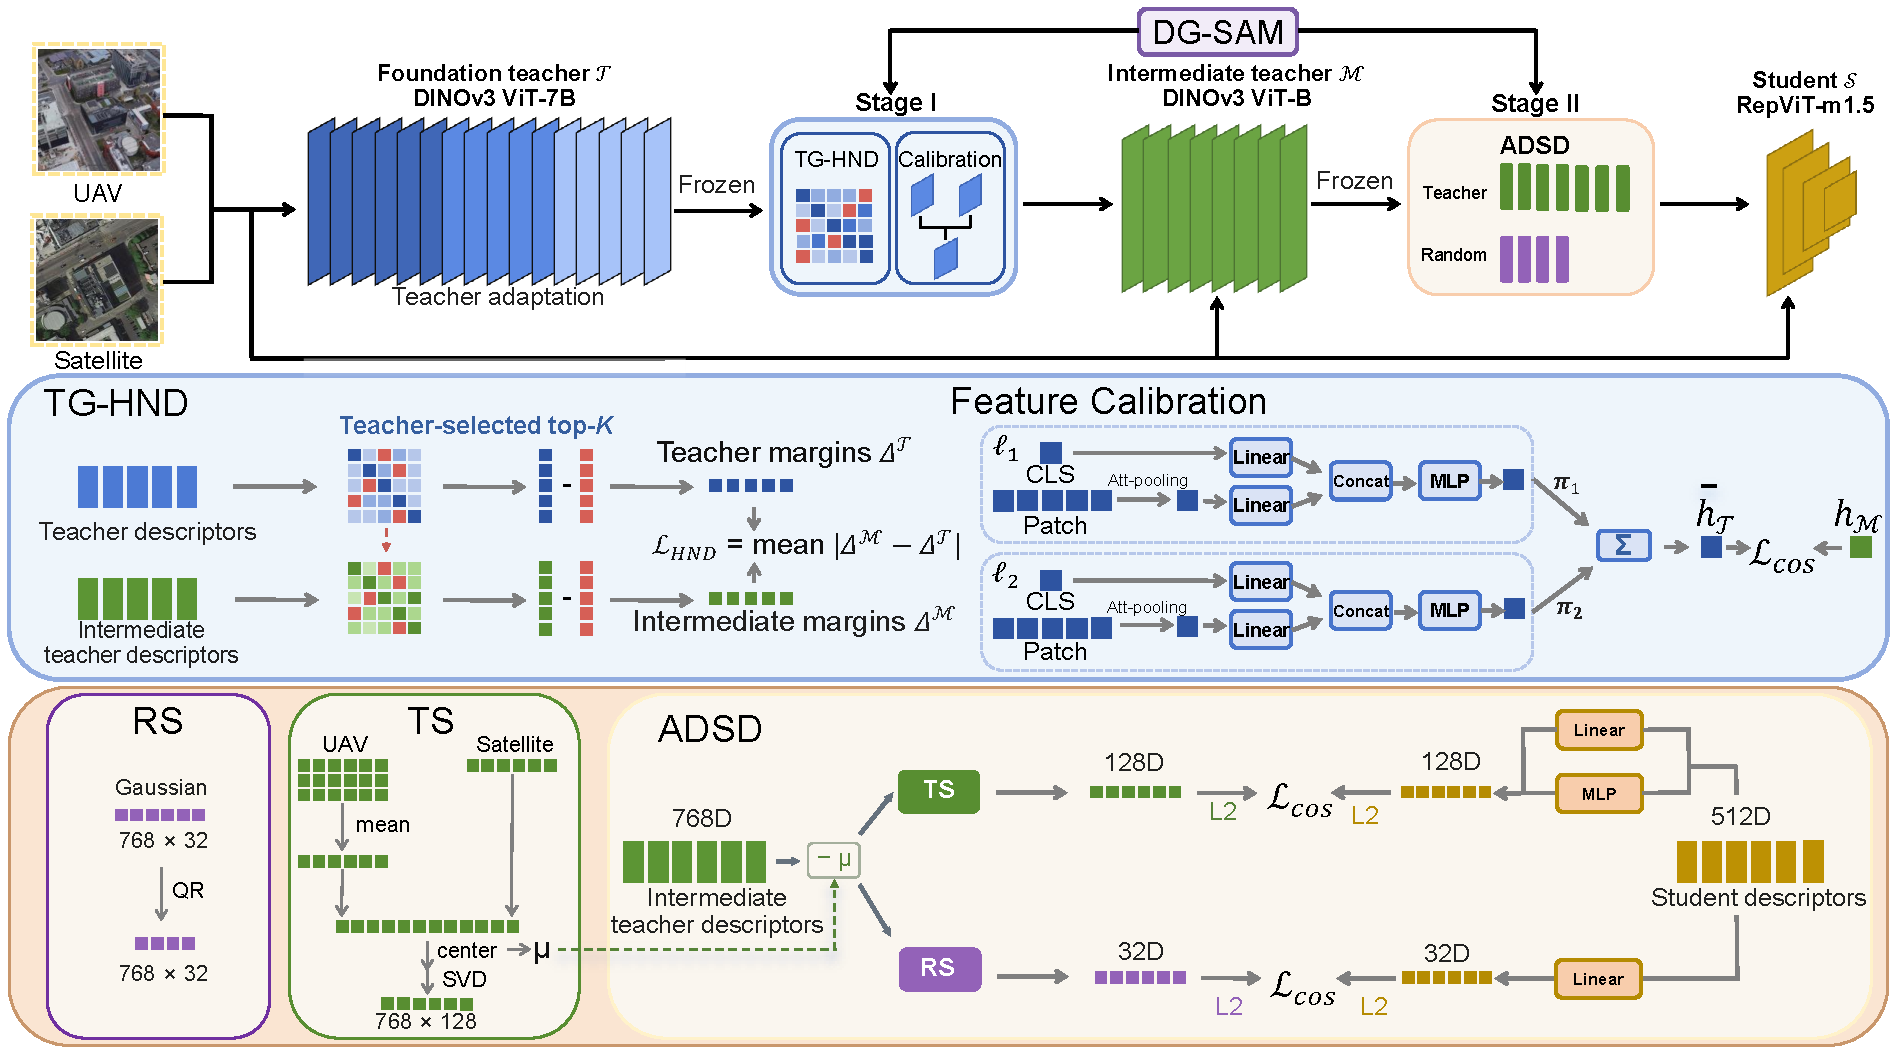
\includegraphics[width=0.96\textwidth]{figure2-128-32.pdf}
\caption{Overview of EfficientGeo. Stage~I uses TG-HND and auxiliary feature calibration for cross-capacity transfer. Stage~II uses ADSD for cross-architecture transfer through the PCA-based Teacher Subspace (TS) and an independently sampled Random Subspace (RS).}
\label{fig:framework}
\end{figure*}


\paragraph{Retrieval objective.}
For the encoder being trained, let
$C\in\mathbb{R}^{N\times N}$ be its UAV-to-satellite
similarity matrix, where
$C_{ij}=z(x_i^u)^\top z(x_j^s)$. The diagonal entry
$C_{ii}$ corresponds to a positive pair, while
$C_{ij}$ with $j\ne i$ corresponds to a negative pair.

For the two retrieval directions
$\omega\in\{u\rightarrow s,s\rightarrow u\}$, we use
$C^{u\rightarrow s}=C$ and
$C^{s\rightarrow u}=C^\top$. Thus, $C_{ij}^{\omega}$
is the similarity between query $i$ and candidate $j$
in direction $\omega$.

Let $\tau>0$ be a learnable temperature and
$q_{ij}=(1-\eta)\mathbf{1}[i=j]+\eta/N$ be the target
probability, where $\eta$ is the label-smoothing factor.
The bidirectional InfoNCE loss~\cite{deuser2023sample4geo}
is
\begin{equation}
\mathcal{L}_{\mathrm{ret}}
=-\frac{1}{2N}
\sum_{\omega}\sum_{i,j=1}^{N}
q_{ij}
\log
\frac{\exp(C_{ij}^{\omega}/\tau)}
{\sum_{k=1}^{N}\exp(C_{ik}^{\omega}/\tau)}.
\label{eq:retrieval}
\end{equation}
We use this loss to adapt $\mathcal{T}$ and to train
$\mathcal{M}$ and $\mathcal{S}$ in Stages~I and~II,
respectively. When needed, a superscript on
$\mathcal{L}_{\mathrm{ret}}$ identifies the corresponding
model. Each model has its own temperature. We set
$\eta=0$ for $\mathcal{T}$ and $\mathcal{M}$, and
$\eta=0.1$ for $\mathcal{S}$.

\paragraph{Teacher adaptation.}
Before distillation, we adapt pretrained DINOv3 ViT-7B
using $\mathcal{L}_{\mathrm{ret}}^{\mathcal{T}}$.
We freeze its early Transformer blocks, apply
LoRA~\cite{hu2022lora} to intermediate blocks, and
fully fine-tune the final blocks. Further implementation details are provided in Section A.1 of the supplementary material.

\subsection{Teacher-Guided Hard Negative Distillation}
\label{sec:tghnd}

\paragraph{Teacher-guided margin transfer.}
For query $i$ and retrieval direction $\omega$, let
$C_{\mathcal{T}}^\omega$ and
$C_{\mathcal{M}}^\omega$ be the similarity matrices of
$\mathcal{T}$ and $\mathcal{M}$, respectively. The teacher
selects the indices $\mathcal{H}_i^\omega$ of its $K=5$
highest-scoring in-batch negatives. The positive--negative
margin measures the similarity gap between the positive
candidate $i$ and a selected negative candidate $j$:
\begin{equation}
\mathcal{H}_i^\omega
=\operatorname{TopK}_{j\ne i}
C_{\mathcal{T},ij}^\omega,
\qquad
\Delta_{ij}^\omega
=C_{ii}^\omega-C_{ij}^\omega.
\label{eq:hnd_candidates_margins}
\end{equation}
We write $\Delta_{\mathcal{T},ij}^\omega$ and
$\Delta_{\mathcal{M},ij}^\omega$ for the margins computed
by the teacher and intermediate model, respectively.
We align these margins on the selected negatives:
\begin{equation}
\mathcal{L}_{\mathrm{HND}}
=\frac{1}{2NK}
\sum_{\omega}
\sum_{1\leq i\leq N}
\sum_{j\in\mathcal{H}_i^\omega}
\left|
\Delta_{\mathcal{M},ij}^\omega
-\Delta_{\mathcal{T},ij}^\omega
\right|.
\label{eq:hnd_loss}
\end{equation}

\paragraph{Auxiliary multi-level feature calibration.}
To complement margin transfer, we extract the
classification (CLS) token and patch tokens from two
selected layers of $\mathcal{T}$ for each image $x$.
At each layer, attention pooling summarizes the patch
tokens, and a layer-specific bridge combines the pooled
feature with the CLS token and maps it to the
hidden-feature dimension of $\mathcal{M}$. Let
$\mathbf{h}_{\mathcal{T}}^{(1)}(x)$ and
$\mathbf{h}_{\mathcal{T}}^{(2)}(x)$ be the resulting
features. The fused teacher target is
\[
\bar{\mathbf{h}}_{\mathcal{T}}(x)
=\pi_1\mathbf{h}_{\mathcal{T}}^{(1)}(x)
+\pi_2\mathbf{h}_{\mathcal{T}}^{(2)}(x),
\]
where $\pi_1$ and $\pi_2$ are learned, softmax-normalized
weights shared across images and views.

Let $\mathbf{h}_{\mathcal{M}}(x)$ be the CLS feature from
a selected hidden layer of $\mathcal{M}$. For
$i=1,\ldots,N$ and $v\in\{u,s\}$, we align it with
the fused teacher target using a cosine loss:
\begin{equation}
\mathcal{L}_{\mathrm{cal}}
=\frac{1}{2N}\sum_{i,v}
\left[
1-\cos\left(
\mathbf{h}_{\mathcal{M}}(x_i^v),
\bar{\mathbf{h}}_{\mathcal{T}}(x_i^v)
\right)
\right].
\label{eq:calibration_loss}
\end{equation}
The calibration modules are trained jointly with $\mathcal{M}$.
Bridge details are provided in Section A.3 of the supplementary material.

The Stage~I objective is
\begin{equation}
\mathcal{L}_{\mathrm{I}}
=\mathcal{L}_{\mathrm{ret}}^{\mathcal{M}}
+\lambda_{\mathrm{HND}}\mathcal{L}_{\mathrm{HND}}
+\lambda_{\mathrm{cal}}\mathcal{L}_{\mathrm{cal}}.
\label{eq:stage_one_objective}
\end{equation}


\subsection{Asymmetric Dual-Subspace Distillation}
\label{sec:adsd}
\paragraph{Dual-subspace target construction.}
To supervise $\mathcal{S}$, we project the descriptors of
$\mathcal{M}$ onto a Teacher Subspace (TS) and a Random
Subspace (RS). For each training location, the UAV centroid is obtained
by averaging the descriptors of its unaugmented UAV images
and $\ell_2$-normalizing the result, while the satellite
centroid is the descriptor of its single unaugmented
satellite image. Let $\mu$ be the mean of
these centroids.
We apply principal component analysis (PCA) to the
centered centroids and use the leading directions as the
TS basis $P$. Independently, we orthonormalize Gaussian
vectors to obtain the RS basis $R$. The two bases are not
constrained to be mutually orthogonal. Both bases and
$\mu$ remain fixed during student training. 
Further details of the centroid and subspace construction
are provided in the supplementary material.

For an augmented image $x$, $\mathcal{M}$ produces the
descriptor $z_{\mathcal{M}}(x)$. The two targets for
$\mathcal{S}$ are
\begin{equation}
\begin{aligned}
t_p(x)&=\operatorname{norm}\!\left(
P^\top[z_{\mathcal{M}}(x)-\mu]\right),\\
t_r(x)&=\operatorname{norm}\!\left(
R^\top[z_{\mathcal{M}}(x)-\mu]\right),
\end{aligned}
\label{eq:adsd_targets}
\end{equation}
where $\operatorname{norm}(\cdot)$ denotes
$\ell_2$ normalization.

\paragraph{Asymmetric student mappings.}
For the same image $x$, $\mathcal{S}$ produces the
descriptor $z_{\mathcal{S}}(x)$. The student predictions
corresponding to TS and RS are
\begin{equation}
\begin{aligned}
\hat{t}_p(x)&=\operatorname{norm}\!\left(
W_pz_{\mathcal{S}}(x)+b_p
+\gamma f(z_{\mathcal{S}}(x))\right),\\
\hat{t}_r(x)&=\operatorname{norm}\!\left(
W_rz_{\mathcal{S}}(x)+b_r\right),
\end{aligned}
\label{eq:adsd_student_heads}
\end{equation}
where $W_p,W_r$ and $b_p,b_r$ are the weights and biases
of the linear mappings, $f$ is a learnable two-layer
multilayer perceptron (MLP) with Gaussian error linear
unit (GELU) activation, and $\gamma$ is a learnable scalar.
Both mappings are shared across views, with initialization
details provided in the supplementary material.

For $k\in\{p,r\}$, $i=1,\ldots,N$, and $v\in\{u,s\}$,
we align each student prediction with its corresponding
teacher target using a cosine loss:
\begin{equation}
\mathcal{L}_k
=\frac{1}{2N}\sum_{i,v}
\left[
1-\cos\left(\hat{t}_k(x_i^v),t_k(x_i^v)\right)
\right].
\label{eq:adsd_branch_loss}
\end{equation}

\paragraph{Branch weighting.}
Gradient-balanced weighting (GBW) uses a separately
optimized gate to adjust the branch weights $w_p$ and
$w_r$, encouraging the weighted gradient norms of the
two losses with respect to the shared student descriptor
to be similar. Further details of the gate objective and
gradient computation are provided in Section A.4 of the supplementary
material.

The Stage~II objective is
\begin{equation}
\mathcal{L}_{\mathrm{II}}
=\mathcal{L}_{\mathrm{ret}}^{\mathcal{S}}
+\lambda_{\mathrm{ADSD}}\!\left(
w_p\mathcal{L}_p+w_r\mathcal{L}_r
\right).
\label{eq:stage_two_objective}
\end{equation}
The distillation weight $\lambda_{\mathrm{ADSD}}$ increases
from $0.04$ to $0.2$ in steps of $0.04$ over the first five
epochs and remains fixed thereafter.

\subsection{Optimization and Inference}
\label{sec:optimization}

\paragraph{Distillation-guided optimization.}
To encourage more stable knowledge transfer under parameter
perturbations, we apply distillation-guided sharpness-aware
minimization (DG-SAM) in both stages, based on
SAM~\cite{foret2021sam}. DG-SAM constructs the perturbation
using only the distillation terms in each stage objective.

Let $g_{\mathrm{KD}}$ denote the gradient of the weighted
distillation terms in the current stage objective: TG-HND
and feature calibration in Stage~I
(Eq.~\eqref{eq:stage_one_objective}), and ADSD in Stage~II
(Eq.~\eqref{eq:stage_two_objective}). The gradient is taken
with respect to the trainable parameters $\phi$ of the
recipient model and its auxiliary modules. The resulting
perturbation is
\begin{equation}
\varepsilon_{\phi}
=\rho\frac{g_{\mathrm{KD}}}
{\|g_{\mathrm{KD}}\|_2+\delta},
\label{eq:dgsam_perturbation}
\end{equation}
where $\rho=0.1$ controls the perturbation magnitude and
$\delta=10^{-12}$ ensures numerical stability.

On the same batch, we compute the gradient of the complete
stage objective, including both retrieval and distillation,
at $\phi+\varepsilon_{\phi}$, treating the perturbation as
fixed. We then restore $\phi$ and update it using this
gradient. The separately optimized GBW gate in Stage~II is
excluded from the perturbation. Further details of the
DG-SAM update are provided in Section A.5 of the supplementary material.

\paragraph{Inference.}
At inference, the student $\mathcal{S}$ uses the same
RepViT-M1.5 encoder~\cite{wang2024repvit} for both UAV
and satellite images, producing 512-dimensional descriptors.
Gallery images are ranked by cosine similarity between their
descriptors and the query descriptor. For deployment, RepViT's
native structural reparameterization can be applied while
retaining the post-pooling batch normalization.
